% !TeX root = ../Thesis.tex

\chapter{Neues Konzept} \label{ch:NewMethods}
%Describe your new methods/procedure (mathematically, conceptually, comprehensibly). Change the title of this chapter if there is a term for your new methods.
\section{Überblick}
\begin{figure}[h]
  \centering
  \includegraphics[width=0.99\linewidth]{Figures/graphAbstract.png}
  \caption{Graphical Abstract - Das Ablaufdiagramm stellt den Prozess dar, durch den das Segmentierungsnetz gewählt wird, das für die Anwendung der vorliegenden Arbeit eingesetzt wird. 
  Ein peer-reviewed Benchmark Datensatz aus Bildern von diversen Zellkulturen mit dazugehörigen Ground Truths wird links eingegeben. 
  Mehrere austauschbare Segmentierungsnetze führen eine Inferenz für den Benchmark aus, zwischen den entstehenden Segmentierungsmasken und den Ground Truths werden dann Übereinstimmungen gesucht. 
  Aus diesen Korrespondenzen, den Metadaten und den Masken wird die neu eingeführte IPQ (siehe \ref{sec:Kriterien}) berechnet. 
  Mithilfe der Ergebnisse kann dann das optimale Segmentierungsnetz für die Anwendung gewählt werden.}
  \label{fig:graph_abstract}
\end{figure}
Das nachfolgende Kapitel beschreibt und diskutiert das angewandte Konzept der vorliegenden Thesis im Detail. 
Es behandelt vor allem die selbstentwickelten Beiträge zu den Methoden. 
Mit dem Kapitel sollen alle Verfahren und deren Bewertung klar verständlich sein.

\section{Bewertungskriterien}\label{sec:Kriterien}
Zur Wahl des Segmentierungsnetzes wird ein neues Bewertungskriterien eingeführt und auf einem annotierten Datensatz getestet.
Als Datensatz wird der S-BIAD1518 \cite{Kromp2020_Dataset, chen20223_Dataset} genutzt, da dieser nicht in den Trainingsdaten eines der Segmentierungsnetze vorkommt.
Im Gegensatz zu selbstentwickelten synthetischen Daten weicht die Bilddomäne dieses Benchmarks zwar stärker von der Domäne der Zieldaten ab,
aber dafür sind die Daten an eine Veröffentlichung mit standardisiertem Peer-Review-Prozess gebunden.
Das Kriterium ist eine Abwandlung der \ac{pq} \cite{kirillov2019PQ}, die hier \ac{ipq} genannt wird. 
Ziel dabei ist es, zum einen, durch standard \ac{pq} die \ac{iou} für individuelle Instanzen zu bewerten und \ac{fp} sowie \ac{fn} Detektionen zu bestrafen. 
Zum anderen sollen Verletzungen der injektiven Abbildung von segmentierten Nuclei auf die Instanzen der \ac{gt} negativ bewertet werden, da die Anzahl der Nuclei eine bedeutungsvoll Metrik für den Nutzer ist. 
Für die Berechnung wird im ersten Schritt der nachfolgende Brute Force Algorithmus angewandt, der die Zuordnung von Segmentierungsinstanzen zu \ac{gt}-Instanzen durchführt.

\begin{algorithm}
\caption{Beste \ac{gt}-Zuordnung für jede Segmentierungsinstanzen}
\begin{algorithmic}
\REQUIRE $mask_\text{prediction}$, $mask_\text{groundTruth}$
\ENSURE $gt_\text{opt}$, $IoU_\text{opt}$

%\STATE $gt\_ids \gets \{ mask_\text{groundTruth} \neq 0 \}$
%\STATE $pred\_ids \gets \{ mask_\text{prediction} \neq 0 \}$
%\STATE $IoU_\text{opt} \gets [0]$
%‚\STATE $gt_\text{opt} \gets [0]$

\FOR{$id_\text{blob}$ in $|mask_\text{prediction}|$}
  \STATE $blob \gets mask_\text{prediction}[id_\text{blob}]$
  %\STATE $IoU_\text{opt}[i] \gets 0$
  %\STATE $gt_\text{opt}[i] \gets 0$

  \FOR{$gt$ in $mask_\text{groundTruth}$}
     \STATE $IoU \gets IoU(gt, blob)$
%    \STATE $gt\_blob \gets mask_\text{groundTruth} == gt\_id$
%    \STATE $intersection \gets \sum (pred\_blob \wedge gt\_blob)$
%    \STATE $union \gets \sum (pred\_blob \vee gt\_blob)$
%    \STATE $iou \gets intersection / union$ wenn $union > 0$ sonst $0$

    \IF{$iou > IoU_\text{opt}[id_\text{blob}]$}
      \STATE $IoU_\text{opt}[id_\text{blob}] \gets iou$
      \STATE $gt_\text{opt}[id_\text{blob}] \gets gt\_id$
    \ENDIF
  \ENDFOR
\ENDFOR

\RETURN $gt_\text{opt}$, $IoU_\text{opt}$
\end{algorithmic}
\end{algorithm}

Die nachfolgende Formel zeigt das \ac{ipq} Bewertungskriterium unterteilt in die 3 Aufgaben:
\begin{equation}
\text{IPQ} = 
\underbrace{
\frac{k_1 \times \displaystyle\sum_{(p, g) \in TP} 
\text{IoU}\left(\displaystyle\bigcup_{p_i \in p} p_i,\, g\right)
}{|TP|}
}_{\text{Segmentatierungs-Qualität (SQ)}}
\times
\underbrace{
\frac{k_2\times|TP|}{|TP| + \frac{1}{2}|FP| + \frac{1}{2}|FN|}
}_{\text{Recognition Qualität (RQ)}}
\times
\underbrace{
\frac{k_3\times\displaystyle |GT|}{\displaystyle\sum_{p \in P} \left( \max(1, n_p - 1) \right)} }_{\text{Injektivitäts-Qualität (IQ)}},
\end{equation}\label{eq:ipq}
wobei:
\begin{itemize}
    \item $k_1, k_2, k_3$ Optionale Vorfaktoren zur Gewichtung der drei Teile der Metrik sind.
    \item $TP$ die Menge aller \ac{tp}-Tupel $(p, g)$ ist, wobei $g$ eine \ac{gt}-Instanz und $p$ der Vektor aller zugehörigen Segmentierungsinstanzen ist.
    \item $|TP| \in \mathbb{Z}$ die Anzahl an korrekt erkannten Instanzen bezeichnet, also \ac{gt}-Instanzen mit $\text{IoU} > 0{,}5$.
    \item \ac{iou}$(\bigcup_{p_i \in p}p_i, g) \in [0,1] $ die \ac{iou} zwischen der allen Segmentierungsinstanzen $p_i$ in der \ac{tp}-Instanz \textit{p} und der zugehörigen \ac{gt}-Instanz \textit{g} beschreibt.   
    \item $|FP| \in \mathbb{Z}$ die Anzahl an falsch-positiven Segmentierungen ist, d.\,h. vorhergesagte Instanzen ohne \ac{gt}-Entsprechung.
    \item $|FP| \in \mathbb{Z}$ die Anzahl an nicht erkannten \ac{gt}-Instanzen ist, also \ac{gt}-Instanzen ohne zugehörige Vorhersage.
    \item $|GT| \in \mathbb{Z}$ die Anzahl der \ac{gt}-Instanzen ist.
    \item $P$ die Menge aller Segmentierungsinstanzen ist, ungeachtet der \ac{gt}-Zuordnung.
    \item $p \subseteq P$ ein Vektor aller Segmentierungsinstanzen, die der gleichen \ac{gt}-Instanz zugeordnet sind, ist.
    \item $n_p$ die Dimension des Vektors $p$ ist.
    \item $\text{SQ} \in [0,1]$ ein Faktor ist, der die Qualität der Segmentierung anhand der \ac{iou} von der segmentierten und der erwarteten Instanz vergleicht.
    \item $\text{RQ} \in [0,1]$ ein Faktor ist, der bewertet, wie vollständig und das Segmentierungsnetz die vorhandenen Nuclei gefunden hat und, ob es dabei zu Halluzinationen kam.
    \item $\text{IQ} \in [0,1]$ ein Faktor ist, der das Unterteilen von Nuclei durch das Segmentierungsnetz zu bestrafen. Wird ein Nucleus durch mehrere Instanzen der Segmentierungsmaske dargestellt, wird $n_p$ größer als Eins und der Faktor sinkt.
    \item $\text{IPQ} \in [0,1]$ ein Maß für die panoptische Segmentierungsqualität mit der Voraussetzung von injektiver Abbildung der Segmentierungsmasken-Instanzen auf die \ac{gt}-Instanzen darstellt, wobei höhere Werte bessere Übereinstimmung bedeuten.
\end{itemize}

\section{Klassifikator}
Jedem instanzsegmentierten Nuclei muss eine Klasse zugewiesen werden, um die Ausgabe zur panoptischen Segmentierungsmaske zu erweitern.
Hierzu ist ein Klassifikator notwendig, der einen Bildausschnitt mit der Instanz als Eingabe annimmt und eine der vier Klassen als Ausgabe zuweist.
Um diesen Klassifikator optimal zu erstellen wird ein umfangreicher Benchmark aus den Zieldaten erstellt, da bei der Messung der Klassifikationsleistung eine vollkommene Übereinstimmung der Bilddomäne notwendig ist.
Benchmarks aus der Literatur umfassen weder dieselben Klassen noch dieselben Objektmerkmale und eignen sich daher nicht.
Für das Training wird einheitlich der Adam Algorithmus \cite{Kinga2015} mit einer Lernrate von 0.0001 eingesetzt.
Außerdem wird der Cross-Entropy-Loss \cite{Sukhbaatar2014} verwendet. \textbf{ * Notiz: muss ich das erklären? (in der Theorie dann) *} \newline
Aus den annotierten Bilddaten werden für jede Anwendung ein Test- und ein Trainingsanteil im Verhältnis eins zu neun extrahiert.
Alle betrachteten Variationen des Klassifikators werden ausschließlich mit den Trainingsdaten trainiert und ihre Leistung ausschließlich mithilfe der Testdaten getestet.
Beide Anteile des Datensatzes werden durch Augmentierung erweitert und in Batches zusammengefasst.
Zur Datenaugmentierung werden die folgenden Methoden eingesetzt:
\begin{itemize}
  \item \textbf{Rotation:} Mit einer Wahrscheinlichkeit von 50\,\% werden die Eingabedaten um 90° in der XY-Ebene rotiert.
  \item \textbf{Spiegelung:} Ebenfalls mit einer Wahrscheinlichkeit von 50\,\% erfolgt eine Spiegelung entlang der Z-Achse.
  \item \textbf{Gaußsches Rauschen:} Mit einer Wahrscheinlichkeit von 20\,\% wird Rauschen mit einem Mittelwert von 0 und einer Standardabweichung von 0{,}01 hinzugefügt.
\end{itemize}
Prominente Encoder aus der Literatur werden vergleichen eingesetzt. 
Darüber hinaus werden hier verschiedene Methoden der Vorverarbeitung, des Vortraining und der Decoder-architektur eingeführt und verglichen.
Im Folgenden sind diese Methoden einzeln beschrieben.
Da jede mögliche Kombination mit jedem Netz zu trainieren einen zu hohen Rechenaufwand bedeuten würde, wird eine Vorauswahl von Kombinationen getroffen. \newline 

%Es werden sowohl \ac{cnn} als auch Vision Transformer basierte Klassifikatioren in Betracht gezogen.
\subsection{Encoder}
Tab. \ref{tab:network_comparison} zeigt die verschiedenen Encoder, die hier eingesetzt werden.
Bis auf das Segmentierungsmodell CellposeSAM handelt es sich dabei um Encodern, die aus Klassifikator Applikationen, die auf dem ImageNet Datensatz \cite{Russakovsky2015} vortrainiert wurden, stammen.  
In der Tabelle sind die Namen, Anzahl der Parameter und, falls vorhanden, die Top-1-Genauigkeit (Acc@1) und die Top-5-Genauigkeit (Acc@5) auf dem ImageNet Datensatz angegeben.
\begin{table}[ht]
  \centering
  \caption{Vergleich der sechs vortrrainierten Netze hinsichtlich Genauigkeit auf dem ImageNet Datensatz \cite{Russakovsky2015} und der Anzahl an Parametern.
  Angegeben sind sowohl die Top-1-Genauigkeit (Acc@1) als auch die Top-5-Genauigkeit (Acc@5), also  ob die korrekte Klasse unter den besten 1 bzw. 5 Vorhersagen enthalten ist.}
  \label{tab:network_comparison}
  \begin{tabular}{lccc}
    \hline
    \textbf{Name} & \textbf{Acc@1 (ImageNet)} & \textbf{Acc@5 (ImageNet)} & \textbf{Params (M)} \\
    \hline
    ResNet18	      & 69.76\%	& 89.08\% &	11.7 \\
    ResNet101	      & 77.37\%	& 93.55\% &	44.5 \\
    Swin V2	        & 84.11\%	& 96.87\% &	87.9 \\
    ConvNeXt	      & 84.41\%	& 96.98\% &	197.8 \\
    EfficientNet V2 &	85.81\%	& 97.79\% &	118.5 \\
    CellposeSAM	    & -       &	-       &	305 \\
    \hline
  \end{tabular}
\end{table}

\subsection{Vorverarbeitung}
Da in vielen Bildausschnitten Nuclei sehr nah aneinander liegen und dem Klassifikator signalisiert werden muss, welcher der sichtbaren Nuclei klassifiziert werden soll, werden für jeden Klassifikator zwei verschiedene Eingangsdaten-Formate getestet.
Diese Typen unterscheiden sich in der Art, wie die Segmentierungsmaske des zu klassifizierenden Nucleus dem Klassifikator zugänglich gemacht wird.
%Für Daten des ersten Typs wird lediglich der minimale Begrenzungsrahmen des segmentierten Nucleus aus dem originalen Nucleus Kanal ausgeschnitten. 
Daten des ersten Typs ersetzenden Nucleus-Kanal, mit der Segmentierungsmaske des gesuchten Nucleus.
Das Ziel ist dabei das Risiko zu minimieren, dass umliegende Nuclei das Klassifikationsergebnis verfälschen.
Mit dieser Risikominimierung geht allerdings der Verlsut der Oberflächenmerkmale einher.
Außerdem ist das Klassifikationsergebnis bei dieser Vorverarbeitungsart von der Qualität der Segmentierung abhängig.
%Alle anderen Kanäle, einschließlich des Nuclei Kanal bleiben unverändert.
Für Daten des Typ zwei wird der Nucleus-Kanal mit einer Entfernungsmaske skaliert.
Hierzu wird pixelweise der originale Nucleus-Kanal mit einer Transformation des Abstand aller Pixel außerhalb der Segmentierungsmaske wie folgt multipliziert:
\begin{equation}
I'(x) = I(x) \cdot \exp\left( -\frac{1}{\sigma} \min_{y \in \lnot M} \|x - y\|_2 \right),
\label{eq:distance}
\end{equation}
wobei:
\begin{itemize}
  \item $\quad I(x) \in [0, 1]$ der Intensitätswert des Nucleus Kanal an der Position $x$ ist,
  \item $\quad I'(x)  \in [0, 1]$ der Intensitätswert des neuen, transformierten Nucleus Kanal an der Position $x$ ist,
  \item $\quad x \in \Omega \subset \mathbb{N}^3$ die Position eines Voxels im diskreten Bildraum ist,
  \item $\quad M \subseteq \Omega$ die Segmentierungsmaske und $\lnot M = \Omega \setminus M$ deren Komplement im Bildraum sind,
  \item und $\sigma \in \mathbb{R}^+$ ein Parameter zur Steuerung des exponentiellen Abfalls ist.
\end{itemize}
Die Verwendung des Typ zwei hat zum Ziel, dass die Oberflächenmerkmale des Nucleus erhalten bleiben.
Außerdem wird mit der Vorverarbeitung des zweiten Typs der Einfluss den eventuelle fehlerhafte Segmentierungsmasken haben durch die kontinuierliche Abstandstransformation minimiert.
Allerdings ist hierdurch auch das Risiko von Einflussnahme auf das Klassifikationsergebnis durch umliegende Nuclei nicht vollständig eliminiert, sondern nur vermindert.
Im Folgenden sind die Nuclei Kanäle der verschiedenen Methoden dargestellt.
\begin{figure}[htbp]
  \centering
  % \begin{subfigure}[t]{0.18\textwidth}
  %     \includegraphics[width=\linewidth]{Figures/cutout.png}
  %     \caption{Minimaler Begrenzungsrahmen des Nuclei-Kanals, wie Daten des ersten Typs ihn enthalten.}
  % \end{subfigure}
  % \hfill
  \begin{subfigure}[t]{0.24\textwidth}
      \includegraphics[width=\linewidth]{Figures/VERSION2_CH_0_SLICE_4.png}
      \caption{Ausgeschnittener Bereich des originalen Nucleus-Kanals mit mehreren Nuclei.}
  \end{subfigure}
  \hfill
  \begin{subfigure}[t]{0.24\textwidth}
      \includegraphics[width=\linewidth]{Figures/VERSION1_CH_2_SLICE_4.png}
      \caption{Segmentierungsmaske des zu klassifizierenden Nucleus, wie Daten des ersten Typs sie enthalten.
      Die binäre Maske zeigt keine Oberflächenmerkmale des Nucleus, lediglich die geometrischen Merkmale.}
  \end{subfigure}
  \hfill
  \begin{subfigure}[t]{0.24\textwidth}
      \includegraphics[width=\linewidth]{Figures/VERSION2_CH_2_SLICE_4.png}
      \caption{Entfernungsmaske des zu klassifizierenden Nucleus. 
      Diese wird pixelweise mit dem Nucleus-Kanal multipliziert für Typ zwei.}
  \end{subfigure}
  \hfill
  \begin{subfigure}[t]{0.24\textwidth}
      \includegraphics[width=\linewidth]{Figures/VERSION1_CH_0_SLICE_4.png}
      \caption{Darstellung des Typs zwei, entstanden durch Multiplikation von Nuclei-Kanal und Entfernungsmaske.
      Zu sehen ist, dass der nahegelegene ungewünschte Nucleus noch stellenweise mit hoher Intensität vertreten ist.}
  \end{subfigure}
  \caption{Darstellungen der verschiedenen Typen von Eingangsdaten. Jeder Typ zielt auf eine andere Art darauf ab, dem Klassifikator zu signalisieren, welcher der sichtbaren Nuclei zu segmentieren ist.}
  \label{fig:five_images}
\end{figure}

Je nach Modellarchitektur müssen die Bilddaten noch skaliert werden, bervor sie den vortrainierten Modellen übergeben werden können, da die Klassifikatoren Eingaben konstanter Größe benötigen.
%Hierzu werden zwei Methoden eingeführt und in Experimenten verglichen.
%Die erste Methode ist konventionelles Zero-Padding, also das symetrische Hinzufügen von Nullen an die Ränder des Bilds.
Dazu wird einfache bilineare Interpolation verwendet. \textbf{ *  muss ich das erklären? *} \newline
%Zuletzt wird eine lernbare Methode betrachtet.
%Ein kleines neuronales Netzwerk, vergrößert das Bilder schrittweise. 
%Dabei lernt eine Faltungsschicht zuerst eine Transformation, bevor das Bild mittels bilinearer Interpolation auf die gewünschte Größe hochskaliert wird.

\subsection{Vortraining}
Aus der Literatur sind verschiedene Methoden des Vortraining bekannt.
Hier werden:
\begin{itemize}
  \item Kein Vortraining,
  \item semi-supervised, und
  \item fully-supervised Vortraining 
\end{itemize}
betrachtet.%, sowohl in Kombination, als auch in standalone Umsetzung.
Die Fig. \ref{fig:pretrain} zeigt die hier umgesetzten Methoden.
\begin{figure}[h]
  \centering
  \includegraphics[width=0.8\linewidth]{Figures/PretrainingMethods.png}
  \caption{Übersicht über die Vortrainingsmethoden. 
  Links zu sehen sind die beiden verfügbaren Bildermengen, ImageNet und die Zeildaten.
  Rechts von diesen Bildermengen werden diesen Bildern \ac{gt} Klassen hinzugefügt, entweder durch die ImageNet Datenbank, Experten oder einen Algorithmus.
  Vier verschiedene Versionen jedes Klassifikators werden hier trainiert.
  Das erste Netzwerk wird auf den ImageNet Daten vortrainiert. 
  Anschließend wird mit Experten-Labels der Decoder neu trainiert.
  TODO}
  \label{fig:pretrain}
\end{figure}
\paragraph{Kein Vortraining}
Ohne Vortraining startet der Encoder, der den Großteil der Gewichte umfasst, mit zuffällig initialisierten Werten.
Da diese zufälligen Werte keine sinnvollen Merkmale extrahieren wird ein besonders langes Training mit den Zeildaten durchgeführt.
Jedes Modell wird jeweils für 75 Epochen trainiert.
%\textit{NOTIZ:} Das wird sehr kurz, kann ich das irgendwie anders machen, fällt dir etwas ein?
 
\paragraph{Semi supervised}
Die semi supervised \acp{gt} werden mithilfe eines few-shot gestützen Cluster Algorithmus erstellt.
Ein Experte erstellt hierzu \acp{gt} von wenigen Nuclei.
Danach werden aus den restlichen Segmentierungsmasken einige Merkmale generiert und zu einem Vektor zusammengefasst.
Das Volumen und die Oberfläche und Achsenlängen werden direkt bestimmt. 
Die Exzentrizität wird aus dem Verhältnis der längsten und der kürzesten Achse berechnet.
Für die Kompaktheit wird das Volumen der Maske durch die kleinste mmögliche Begrenzungsbox geteilt.
Darüber hinaus wird aus der Z-Schicht, in der die Segmentierungsmaske am größten ist wird die 2D-Kontur erfasst.
Aus dieser Kontur wird eine komplexe Zahlenfolge berechnet ‚und der Absolutwert der ersten zehn Koeffizienten als einzelne, weitere Merkmale dem Merkmalsvektor hinzugefügt. \newline
Die entstehenden Merkmalsvektoren werden durch eine Standardisierung der Werte, zu einem Mittelwert von Null und Varianz von Eins überführt.
Daraufhin wird eine Hauptkomponentenanalyse (PCA) angewandt, um die Dimensionalität der Merkmalsvektoren auf zehn zu reduzieren und redundante Informationen zu entfernen.
Das Ziel dabei ist es, einen Mittelweg zwischen Informationserhalt und Overfitting-Gefahr sowie Rechenaufwand zu erzielen.
Mithilfe des Label Spreading-Algorithmus mit einer Radial Basis Funktion Kernelfunktion werden die Experten-\acp{gt} über die Struktur der Daten auf die unbeschrifteten Beispiele ausgebreitet.
Durch den Algorithmus entstehen \acp{gt} für die Daten ohne Experten-Labels.
Diese neuen \acp{gt} werden dann eingesetzt, um in 25 Epochen sowohl die Encoder, als auch die Decoder verfügbaren Klassifikatoren zu trainieren.
Optional werden die Gewichte des Encoder hiernach, bis auf die letzten beiden Schichten eingefroren und nur der Encoder wird in weiteren 25 Epochen mit dem Trainingsdatensatz trainiert.
Das Ziel dieses Vorgehens ist es, eine stärkere Generalisierung zu erreichen, indem Overfitting bei der Merkmalsextraktion vermieden wird.
Da der Encoder mit anderen Daten vortrainiert wird, ist zu erwarten, dass er eine sinnvolle Merkmalsextraktion lernt, ohne auf die expliziten Merkmale der individuellen Stichproben im Trainingsdatensatz angewiesen zu sein.
Dadurch sind die Beziehungen zwischen Merkmalen und Klassen, die der Decoder lernt, nicht nur auf die Merkmale des Trainingsdatensatz beschränkt.
\textit{NOTIZ:} Hier soll stehen:
\begin{itemize}
  \item Wie werden "pseudo-labels" mit semi-supervision erstellt?
  \item Wie wird vortrainiert?
  \item Welche Gewichte werden eingefroren?
  \item Wie wird dann Transfertraining durchgeführt?
\end{itemize}

\paragraph{Fully-supervised} %\newline
\textit{NOTIZ:} Hier soll stehen:
\begin{itemize}
  \item Welche Gewichte werden eingefroren?
  \item Wie wird dann Transfertraining durchgeführt?
\end{itemize}
%Das fully-supervised Vortraining der meisten Encoder wird auf dem ImageNet Datensatz \cite{Russakovsky2015} durchgeführt.
%Außerdem wird der vortrainierte Bildencoder von CellposeSAM herangezogen.
%Für das Tra
\subsection{Decoder}
An die Encoder werden jeweils zwei verschiedene Decoder angehängt.
Fig. \ref{fig:classifiers} zeigt die beiden Architekturen systematisch.
Der erste Klassifikator wird hier \textit{Volumen-Klassifikator} genannt.
Er interpretiert die Merkmale, die der Encoder generiert, als Volumen und generiert mithilfe von 3D Faltungen und Pooling eine Repräsentation daraus.
Diese Repräsentation wird dann durch Linear Layers zu vier Ausgabe-Klassen umgeformt.
Die Idee des \textit{Volumen-Klassifikators} ist es, die Merkmale die der Encoder generiert möglichst vollständig zu erfassen und alle räumlichen Beziehungen, auch in Z-Richtung festzustellen.
Hierbei ist das Ziel, dass durch die 3D-Faltungen eine domänenspezifische Interpretation der Merkmale gelernt wird, sodass die neuen Merkmale nach dem anschließenden Pooling aussagekräftig und niederdimensionale sind.
Daneben wird hier der \textit{Schichten-Klassifikator} eingeführt.
Der \textit{Schichten-Klassifikator} betrachtet die einzelnen Schichten des Bilds anhand der individuellen Schichten, die der Encoder ausgibt. 
Dazu werden die räumlichen X und Y Dimensionen durch einen spatial-average zusammengefasst.
Durch eine multihead attention mit vier attention-Köpfen und embedding dimension 256 wird dann eine Repräsentation aus den individuellen Schichten der Merkmale erstellt.
Lineare Layers formen anschließend die Repräsentation zu den vier Klassen um.
Für den textit{Schichten-Klassifikator} ist das Ziel, dass durch die Vereinfachung der Daten aussagekräftige, schichtenweise Merkmale entstehen und, dass diese räumlich invariant sind, da der betrachtete Nucleus in den Bildfenstern zentriert sind.
\begin{figure}[h]
  \centering
  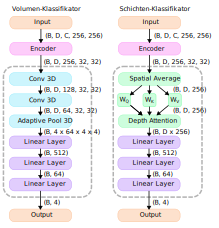
\includegraphics[width=0.9\linewidth]{Figures/Klassifikatoren.png}
  \caption{Architektur der beiden Klassifikatoren. Der Encoder wird bei beiden modular ausgetauscht. 
  Links zu sehen ist die Architektur des \textit{Volumen-Klassifikator}, der die Merkmale, die der Encoder generiert, als Volumen interpretiert und mithilfe von 3D Faltungen und Pooling daraus eine Repräsentation generiert.
  Diese Repräsentation wird dann durch Linear Layers zu vier Ausgabe-Klassen umgeformt.
  Rechts zu sehen ist der \textit{Schichten-Klassifikator}.
  Die räumlichen X und Y Dimensionen werden im \textit{Schichten-Klassifikator} durch einen spatial-average zusammengefasst.
  Durch eine multihead attention mit vier attention-Köpfen und embedding dimension 256 wird dann eine Repräsentation aus den individuellen Schichten der Merkmale erstellt.
  Lineare Layers formen anschließend die Repräsentation zu den vier Klassen um.}
  \label{fig:classifiers}
\end{figure}
\newline
Auf einem geringfügigen Datensatz werden alle angeführten Methoden in den möglichen Kombinationen umgesetzt, um Vergleiche zu ermöglichen.
Dieser geringfügige Datensatz besteht aus Bildern der Zieldomäne und halb automatisch generierten \acp{gt}. 
Anschließend werden die besten Methoden ausgewählt und auf den finalen Datensatz trainiert.
